%
% Quantum Algorithms
%

\section{Quantum algorithms} \index{Quantum algorithms}\label{sec:quantum_algs}

\dropcap{T}{he} ultimate goal of quantum computing is to implement algorithms with a quantum speedup compared to classical algorithms. The degree of speedup achieved varies between algorithms, and it is important to note that not every classical algorithm exhibits any speedup when implemented quantum mechanically.

To provide context for the excitement of quantum computing and motivate interest in their development, we now summarise some of the key quantum algorithms that have been described exhibiting quantum speedup.

%
% Deutsch-Jozsa
%

\subsection{Deutsch-Jozsa} \index{Deutsch-Jozsa algorithm}

The first quantum algorithm demonstrating a provable improvement over the best classical algorithm was the Deutsch-Jozsa algorithm\cite{bib:DeutschJozsa92}. Unfortunately the algorithm solves a very contrived problem, designed for the purposes of demonstrating post-classicality rather than solving a problem of actual practical interest. Nonetheless, the algorithm is straightforward to explain and understand, making it a useful starting point in understanding quantum algorithms and the computational enhancement they may offer.

The algorithm relies on a `black box', referred to as an \textit{oracle}\index{Oracles}, which takes an input bit-string and outputs a single bit, evaluating the function $f(x)$ for the $n$-bit input bit-string $x$. In this contrived problem $f(x)$ is guaranteed to be either \textit{uniform}\index{Uniform function} or \textit{balanced}\index{Balanced function}. In the former case, the output to the oracle is always \mbox{$f(x)=0$} or always \mbox{$f(x)=1$}, but it doesn't matter which, they simply must always be the same. In the latter case, the output is \mbox{$f(x)=0$} for exactly half the inputs $x$, and \mbox{$f(x)=1$} for the other half of $x$, but the ordering of which inputs generate which outputs may be arbitrary. The goal of the algorithm is to determine whether $f(x)$ is uniform of balanced using the least number of queries to the oracle.

While it's clear that the dimensionality of the input state space is exponentially large, $2^n$, it is fairly obvious that a trivial \textbf{BPP}\index{BPP} algorithm exists for solving this problem with confidence exponentially asymptoting to unity against the number of oracle queries. We simply evaluate the oracle for randomly chosen inputs. If we measure any occurrences of measurement outcomes that are not all 0 or all 1 we know with certainty that the function must have been balanced. If on the other hand we measure all 0s or all 1s for more than half the input state space $x$, we know with certainty the function was uniform.

However, if the function were balanced, there is the possibility that it might conspire against us to fool us into thinking the function was uniform until we evaluate half plus one of the input states, requiring $O(2^n)$ oracle queries, although this will occur with exponentially low probability against the number of queries. Thus, the algorithm can be approximated with exponential asymptotic certainty in \textbf{BPP}\index{BPP}. But considering the \textit{worst} case\index{Worst case complexity} rather than the \textit{average} case\index{Average case complexity}, we may have to perform an exponential number of evaluations, $O(2^n)$, to know the answer with absolute certainty.

The Deutsch-Jozsa algorithm solves this rather specialised problem in the worst case using only a single quantum evaluation of the oracle.

The algorithm implementing the Deutsch-Jozsa protocol and its circuit diagram are shown in Alg.~\ref{alg:deutsch_jozsa}. The engine room of the algorithm is in the Hadamard transform\index{Hadamard transform}, $\hat{H}^{\otimes n}$, which prepares an equal superposition of all $2^n$ possible input bit-strings $x$, which are then evaluated in superposition by the oracle. To ensure unitarity, the oracle is defined to implement the transformation\footnote{Note that the seemingly more obvious choice of \mbox{$\hat{U}_f\ket{x}=\ket{f(x)}$} is not unitary. This trick of introducing an additional ancillary state to enable unitary construction of arbitrary functions is a common one in quantum algorithm design.},
\begin{align}
	    \hat{U}_f \ket{x}\ket{y} &= \ket{x}\ket{y\oplus f(x)}.
\end{align}
That is, it flips bit $y$ if \mbox{$f(x)=1$} (equivalently addition modulo 2 or an XOR operation). An inverse Hadamard transform subsequently yields a measurement outcome with one of two possibilities:
\begin{itemize}
	\item The 0 and 1 terms outputted from the oracle interfere perfectly constructively, if the function was uniform.
	\item They interfere perfectly destructively, if the function was balanced.
\end{itemize}
Then, with a single-shot measurement of the inverse Hadamard transformed output from the oracle we establish whether $f(x)$ was balanced or uniform with certainty. This exhibits an exponential worst case speedup compared to a randomised classical sampling algorithm (which is classically optimal).

\begin{table}[!htbp]
\begin{mdframed}[innertopmargin=3pt, innerbottommargin=3pt, nobreak]
\texttt{
function DeutschJozsa(f,n):
\begin{enumerate}
    \item Prepare the \mbox{$n+1$}-bit state,
    \begin{align}
    \ket\psi_0 = \ket{0}^{\otimes n}\ket{1}.	
    \end{align}
    \item Apply the \mbox{$n+1$}-bit Hadamard transform,
    \begin{align}
    \ket\psi_1 &= \hat{H}^{\otimes(n+1)}\ket\psi_0 \nonumber \\
    &= \frac{1}{\sqrt{2^{n+1}}} \sum_{x=0}^{2^n-1}\ket{x}(\ket{0}-\ket{1}),	
    \end{align}
    where $x$ denote $n$-bit binary bit-strings.
    \item Apply the unitary oracle, implementing the transformation,
    \begin{align}
    \hat{U}_f \ket{x}\ket{y} &= \ket{x}\ket{y\oplus f(x)},
    \end{align}
    where $\oplus$ denotes addition modulo 2, yielding,
    \begin{align}
    \ket\psi_2 = \hat{U}_f \ket\psi_1.	
    \end{align}
    \item Apply another Hadamard transform,
    \begin{align}
    \ket\psi_3 = \hat{H}^{\otimes n} \ket\psi_2.
    \end{align}
    \item The full evolution is thus given by,
    \begin{align}
    	\ket\psi_\mathrm{out} = (\hat{H}^{\otimes n}\otimes\hat{I}) \cdot \hat{U}_f \cdot \hat{H}^{\otimes (n+1)}\ket{0}^{\otimes n}\ket{1}.
    \end{align}
	\item Measure the first $n$ qubits to determine the probability of measurement outcome $\ket{0}^{\otimes n}$.
	\item This probability is given by,
	\begin{align}
	P_0 = \left| \frac{1}{2^n} \sum_{x=0}^{2^n-1} (-1)^{f(x)} \right|^2.	
	\end{align}
	\item Depending on whether $f(x)$ was uniform or balanced, the alternating sign terms in this sum interfere constructively or destructively, yielding \mbox{$P_0=1$} or \mbox{$P_0=0$} respectively.
	\item Thus, a single measurement outcome suffices to determine whether $f(x)$ was balanced or uniform.
	\item $\Box$
\end{enumerate}
\begin{align}
\Qcircuit @C=1em @R=1.6em {
    \lstick{\ket{0}^{\otimes n}} & \gate{\hat{H}^{\otimes n}} & \multigate{1}{\hat{U}_f} & \gate{\hat{H}^{\otimes n}} & \meter \\
    \lstick{\ket{1}} & \gate{\hat{H}} & \ghost{\hat{U}_f} & \qw & \\
} \nonumber
\end{align}
}
\end{mdframed}
\captionspacealg \caption{Deutsch-Jozsa algorithm for evaluating whether the function $f(x)$ is balanced or uniform, exhibiting exponential worst case speedup compared to the best classical \textbf{BPP} algorithm\index{BPP}.} \label{alg:deutsch_jozsa}
\end{table}

%
% Quantum Search
%

\subsection{Quantum search}\label{sec:quantum_search} \index{Grover's algorithm}

The problem of finding specific entries in unstructured data spaces is a ubiquitous one. This class of \textit{search algorithms} have amongst the broadest applicability of any class of algorithms. Computer scientists have invested excruciating man-hours\index{SJW}\footnote{Presently, most computer science research institutions are equal opportunity employers.} into organising and structuring data so as to minimise the resource overhead (in time and/or space) associated with extracting desired components. However, the methodology for achieving this, and the favourability of associated resource overheads, is highly dependent on the structure of the underlying data, or whether there even is any. To this end, numerous data structures and algorithms have been developed, accommodating for every mutation and variation of the posed problem imaginable. Often, there is a tradeoff between the overheads induced in time and memory, as well as in pre-processing and data structure maintenance requirements.

For example, \textit{hash tables}\index{Hash tables} enable theoretical $O(1)$ lookup times on data with a \textit{key-value pair}\index{Key-value pair} data structure. In a key-value pair each data entry (value) is tagged with a unique identifier (key) used for lookup. The value can observe any structure whatsoever, whereas the key is designed so as to minimise search times. When storing telephone numbers one might represent entries as key-value pairs, where the keys are people's names, and the values their respective telephone numbers. An efficient algorithm for mapping keys to physical memory addresses would imply efficient lookup of telephone numbers by name.

In the absence of a key-value representation one might simply store data in sorted form. However, this requires pre-sorting the entire data space, which may become costly for large data sets, and requires continual rearrangement whenever the data space is modified, making it computationally costly for mutable datasets.

For the end user, who wishes to find data elements, the worst-case data space is one with no order or underlying structure. Suppose we want to find whether a number exists in the telephone directory, but we don't know it's associated name. In this instance, it can easily be seen that the best one can hope for, in terms of algorithmic runtime, is to simply look through the data space brute-force\index{Brute-force} until we find what we are looking for. It is clear that with an unstructured space of $N$ elements, this brute-force search algorithm requires on average $O(N)$ queries to find the desired entry. We call this the \textit{unstructured search problem}.

The brute-force classical algorithm, despite already being technically `efficient' (i.e $O(N)$ linear runtime), could nonetheless become unwieldy for very large datasets. Google doesn't want to exhaustively scan their entire collection of data-centres each time they want to lookup a database element. The quantum search algorithm, first presented by Grover \cite{grover1997quantum}, provides a solution to this problem using only $O(\sqrt{N})$ runtime (oracle queries), a quadratic enhancement. Whilst this falls far short of the exponential quantum enhancement one might have hoped for, which has also shown to be optimal \cite{bennett1997strengths, zalka1999grover}, it is nonetheless still extremely helpful for many purposes, given the broad applications for this algorithm.

We will formulate the quantum search algorithm as an oracular algorithm\index{Oracles}, where the oracle takes as input an $n$-bit string, and outputs 1 if the input matches the entry we are looking for, otherwise 0. This formulation of the problem makes the algorithm naturally suited to solving satisfiability problems (many of which are \textbf{NP}-complete and of great practical interest).

The Grover quantum search algorithm is shown explicitly in Alg.~\ref{alg:quant_search}.

\begin{table}[!htbp]
\begin{mdframed}[innertopmargin=3pt, innerbottommargin=3pt, nobreak]
\texttt{
function Grover(f,n):
\begin{enumerate}
	\item Using a Hadamard transform, prepare the $n$-qubit equal superposition of all $2^n$ logical basis states,
    \begin{align}
    \ket\varphi &= \hat{H}^{\otimes n}\ket{0}^{\otimes n}	 \nonumber \\
    &= \frac{1}{\sqrt{2^n}}\sum_{x = 0}^{2^n - 1}\ket{x},
    \end{align}
    where $x$ denotes a bit-string of length $n$.
	\item The oracle is defined as a unitary black-box, which tags a target element $T$ using a phase-flip,
	\begin{align}
		\hat{U}_T \ket{x} &= (-1)^{f(x)}\ket{x} \nonumber \\
		&= (\hat{I} - 2\ket{T}\bra{T})\ket{x},
	\end{align}
	where $f(x)=\{0,1\}$ is the black-box function determining whether input $x$ is the target element $T$ (\mbox{$f(x)=1$}) or not (\mbox{$f(x)=0$}).
	\item The Grover diffusion operator\index{Grover diffusion operator} is defined to implement,
	\begin{align}
	\hat{U}_s = \hat{I} - 2\ket{T}\bra{T}.
	\end{align}
    \item repeat $O(N)$ times:
    \setlength{\itemindent}{.2in}
    \item $\ket{\varphi_{i+1}} = \hat{U}_s\cdot\hat{U}_T\ket{\varphi_i}$.
    \setlength{\itemindent}{0in}
    \item $\Box$
    \item \comment{What about measurement stage}
\end{enumerate}
}
\end{mdframed}
\captionspacealg \caption{Grover's algorithm for performing a quantum search over an oracle, exhibiting a quadratic quantum enhancement.} \label{alg:quant_search}
\end{table}

%
% Quantum Fourier Transform
%

\subsection{Quantum Fourier transform}\index{Quantum Fourier transform}\label{sec:QFT_alg}

The quantum Fourier transform (QFT) is not an algorithm per se, but rather a unitary operator that finds widespread use in other quantum algorithms. The QFT operator is so ubiquitous that it warrants special treatment.

The QFT matrix simply contains coefficients taken from the discrete Fourier transform (DFT)\index{Discrete Fourier transform}. Specifically, the \mbox{$N\times N$} QFT matrix has elements,
\begin{align}
\hat{\mathrm{QFT}}_{j,k} = \frac{1}{\sqrt{N}} \omega^{(j-1)(k-1)},	
\end{align}
where,
\begin{align}
\omega = e^{\frac{2\pi i}{N}},	
\end{align}
is a complex root of unity. In matrix form the $N$-dimensional QFT is therefore,
\begin{align}
\hat{\mathrm{QFT}}_N = \frac{1}{\sqrt{N}} \left(\begin{matrix}
  1 & 1 & 1 & \dots & 1\\
  1 & \omega & \omega^2 & \dots & \omega^{N-1} \\
  1 & \omega^2 & \omega^4 & \dots & \omega^{2(N-1)} \\
  \vdots & \vdots & \vdots & \ddots & \vdots \\
  1 & \omega^{N-1} & \omega^{2(N-1)} &\dots &\omega^{(N-1)(N-1)}
\end{matrix}\right),
\end{align}
which is symmetric, \mbox{$\hat{\mathrm{QFT}}=\hat{\mathrm{QFT}}^\top$}. Note that all matrix elements are phases with magnitude $1/\sqrt{N}$,
\begin{align}
	|\hat{\mathrm{QFT}}_{i,j}|=\frac{1}{\sqrt{N}}\,\,\forall\, i,j.
\end{align}

Equivalently, in terms of basis state transformations this implements the map,
\begin{align}
	\hat{\mathrm{QFT}} \ket{j} \to \frac{1}{\sqrt{N}}\sum_{k=0}^{N-1} \omega^{jk}\ket{k},
\end{align}
on the $N$ basis states.

Unlike the closely-related Hadamard transform\index{Hadamard transform}, $\hat{H}^{\otimes n}$, which shares many properties with the QFT, the QFT is a highly entangling operation. The QFT of any dimension has an efficient circuit implementation, making it an important subroutine in many algorithms. Specifically, the $n$-qubit QFT (i.e a transformation on $2^n$ amplitudes) requires only $O(n^2)$ elementary gates (Hadamards and CZs). If an approximation of the QFT is sufficient for one's purposes, this can be further reduced to only \mbox{$O(n\,\log \,n)$}.

\comment{Show algorithm box with circuit}

%
% Phase-Estimation
%

\subsection{Phase-estimation}\index{Phase estimation algorithm}\label{sec:phase_est_alg}

The goal of the phase-estimation algorithm \cite{bib:PhaseEstAlg} is to calculate the eigenvalue of a given unitary operator for a given eigenvector of that unitary. Since the eigenvalues of unitary operators are always phases of amplitude 1, we can write,
\begin{align}
	\hat{U}\ket\psi = e^{2\pi i\theta}\ket\psi,
\end{align}
where $\theta$ parameterises the phase of the eigenvalue and $\ket\psi$ is an eigenvector of $\hat{U}$.

The algorithm for this is baked from several ingredients. To implement phase-estimation with $n$ bits of precision, we require:
\begin{itemize}
	\item An $n$-qubit Hadamard transform, $\hat{H}^{\otimes n}$\index{Hadamard transform}.
	\item $n$ controlled-$\hat{U}$s\footnote{Any unitary has a coherently controlled unitary equivalent, of the form $\hat{U}_\mathrm{controlled} = \ket{0}\bra{0}\otimes \hat{\mathbb{I}} + \ket{1}\bra{1}\otimes\hat{U}$. These always have an efficient circuit construction, given $\hat{U}$.}.
	\item An $n$-qubit inverse quantum Fourier transform\index{Quantum Fourier transform}, $\hat{\mathrm{QFT}}_n^\dag$ (Sec.~\ref{sec:QFT_alg}).
\end{itemize}

Alg.~\ref{alg:q_phase_est} shows the circuit implementation of the phase-estimation algorithm. The output is a binary representation of \mbox{$2^n\theta$}, where the precision is determined entirely by the number of qubits in the output register, which can be arbitrarily large in principle.

\begin{table}[!htbp]
\begin{mdframed}[innertopmargin=3pt, innerbottommargin=3pt, nobreak]
\texttt{
function PhaseEstimation($\hat{U}$, $\ket\psi$, $n$):
\begin{enumerate}
	\item For unitary $\hat{U}$ with eigenvector $\ket\psi$ and respective eigenvalue $e^{2\pi i\theta}$, apply the circuit below, on the input state \mbox{$\ket{0}^{\otimes n}\ket\psi$}.
	\item The register of qubits at the output to the QFT encodes $2^n\theta$ in binary representation, where $n$ determines the number of bits of precision in the output.
	\item $\Box$
\end{enumerate}
\begin{align}
\Qcircuit @C=1em @R=1.6em {
    \lstick{\ket{0}} & \gate{\hat{H}} & \qw &\qw & \dots && \ctrl{3} & \multigate{2}{\hat{QFT}^\dag} & \meter \\
    \lstick{\vdots} & \gate{\hat{H}} & \qw &\qw & \dots & & \qw & \ghost{\hat{QFT}^\dag} & \meter \\
    \lstick{\ket{0}} & \gate{\hat{H}} & \ctrl{1} &\qw & \dots && \qw & \ghost{\hat{QFT}^\dag} & \meter \\
    \lstick{\ket{\psi}} & \qw & \gate{\hat{U}^{2^0}} &\qw & \dots & &\gate{\hat{U}^{2^{n-1}}} & \qw & \qw \\
} \nonumber
\end{align}
}
\end{mdframed}
\captionspacealg \caption{Quantum phase-estimation algorithm.} \label{alg:q_phase_est}
\end{table}

The phase-estimation algorithm is not extremely useful as a standalone product, but acts as a necessary subroutine in many important algorithms, such as Shor's algorithm\index{Shor's algorithm} (Sec.~\ref{sec:shors_alg}) and topological data analysis\index{Topological data analysis} (Sec.~\ref{sec:TDA}).

%
% Quantum Simulation
%

\subsection{Quantum simulation} \index{Quantum chemistry}\index{Quantum simulation}\label{sec:quantum_sim_alg}

The field of quantum computation was originally inspired by Feynman's\index{Feynman} observation that quantum systems cannot be efficiently classically simulated, and therefore maybe computers based on quantum principles could handle this problem. Indeed they can, as was shown by \cite{bib:lloyd1996universal}.

It requires little imagination to recognise that the applications for quantum simulation are enormous, given the multitude of quantum systems under active investigation by researchers across countless fields.

Consider a quantum system comprised of a global Hamiltonian, which may be decomposed into smaller local interaction terms,
\begin{align} \label{eq:Ham_sim_Ham}
\hat{H} = \sum_{i=1}^N \hat{H}_i	,
\end{align}
where each $\hat{H}_i$ acts on a subspace of dimension $m_i$ within the larger system. The evolution of the entire system is given by the unitary operator,
\begin{align}
\hat{U} = e^{i\hat{H}t}.
\end{align}
We wish to simulate this evolution.

From the Campbell-Baker-Hausdorff lemma\index{Campbell-Baker-Hausdorff lemma} we can approximate this as,
\begin{align}\label{eq:CBH_lemma}
	\hat{U} \approx \left(e^{i\hat{H}_1\frac{t}{n}}\dots e^{i\hat{H}_N\frac{t}{n}}\right)^n + O\left(\frac{t^2}{n}\right).
\end{align}
This representation effectively decomposes the global evolution into $nN$ discretised stages of,
\begin{align}
	\hat{U}_j = e^{i\hat{H}_j\frac{t}{n}},
\end{align}
each of which operates on an $m_i$-dimensional subspace, and may therefore be directly efficiently implemented as a unitary gate within the circuit model on a quantum computer. 

Clearly the error terms vanish in the limit of \mbox{$n\to\infty$}, whereby the simulation becomes exact. However, this requires an infinite number of gates via infinitesimal discretisation. We would rather approximate the solution using a finite number of gates. It follows from Eq.~(\ref{eq:CBH_lemma}) that for simulation accuracy $\epsilon$, the number of discrete steps scales as,
\begin{align}
n = O\left(\frac{t^2}{\epsilon}\right),
\end{align}
which scales efficiently with the duration of time being simulated and the accuracy of the simulation.

This approach is efficient and applies to any Hamiltonian which may be decomposed into local terms as per Eq.~(\ref{eq:Ham_sim_Ham}). However many other quantum simulation algorithms have since been described for simulating different types of quantum systems with different Hamiltonian structures \cite{bib:JLP, bib:RohdeWavelet15}. The algorithm is summarised in Alg.~\ref{alg:ham_sim}.

\begin{table}[!htbp]
\begin{mdframed}[innertopmargin=3pt, innerbottommargin=3pt, nobreak]
\texttt{
function HamiltonianSimulation($\hat{H}$, $t$, $\epsilon$):
\begin{enumerate}
	\item Hamiltonian to be simulated is of the form,
    \begin{align} \label{eq:Ham_sim_Ham}
\hat{H} = \sum_{i=1}^N \hat{H}_i	,
\end{align}
where $\hat{H}_i$ are local Hamiltonians operating on low-dimensional spaces, and $\hat{H}$ is the global Hamiltonian for the entire system.
\item For each $\hat{H}_i$ construct a quantum circuit implementing the unitary,
\begin{align}
	\hat{U}_j = e^{i\hat{H}_j\frac{t}{n}}.
\end{align}
\item The degree of discretisation, $n$, is chosen according to,
\begin{align}
n = O\left(\frac{t^2}{\epsilon}\right),
\end{align}
where $t$ is evolution time and $\epsilon$ is the accuracy.
\item Apply the circuits for simulating the local Hamiltonians according to the sequence,
\begin{align}
	\hat{U} = \left(\prod_{j=1}^N \hat{U}_j \right)^n.
\end{align}
\item The algorithm has runtime,
\begin{align}
	O\left(\frac{Nt^2}{\epsilon}\right).
\end{align}
\item $\Box$
\end{enumerate}
}
\end{mdframed}
\captionspacealg \caption{Quantum Hamiltonian simulation algorithm.} \label{alg:ham_sim}
\end{table}

%
% Integer Factorisation
%

\subsection{Integer factorisation} \index{Shor's algorithm}\index{Hidden subgroup problem}\label{sec:shors_alg}

\comment{To do - Heliang}

\comment{Mention relationship to hidden subgroup, period-finding, and discrete-log problems}

While this algorithm is known to reside in \textbf{BQP}, it is strongly believed not to be \textbf{BQP}-complete. Similarly, while it is known to reside in \textbf{NP}, it is strongly believed not to be \textbf{NP}-complete, thereby placing it in the `limbo zone' of \textbf{NP}-intermediate complexity.\index{NP \& NP-complete}

%
% Quantum Machine Learning
%

\subsection{Quantum machine learning} \index{Quantum machine learning}

With present-day classical computing power becoming ever more powerful, the desire to employ machine learning algorithms has become immense. Machine learning techniques have become indispensable in many fields. Quantum machine learning has emerged as an exciting application for quantum computing power, to enhance the power of machine learning algorithms. We devote the entirety of Sec.~\ref{sec:quantum_mind} to this topic.

%
% Topological Data Analysis
%

\subsection{Topological data analysis} \index{Topological data analysis}\label{sec:TDA}

The internet currently comprises extraordinary amounts of data, from which useful information must be extracted if this vast amount of data is to be utilised effectively. For example, firms like Google and Facebook must extract meaningful information from their databases of user behaviour in order to make appropriate advertising suggestions. This task is extremely valuable -- a small improvement in a recommendation engine\index{Recommendation engine}, for example, could be worth many millions of dollars in revenue.

Performing analyses like these is extremely computationally challenging when dealing with such enormous datasets as Facebook's user database or Google's website database, so-called \textit{big data analysis}\index{Big data analysis}.

One avenue for the analysis of large, complex datasets is via homology theory\index{Homology theory}, which yields \textit{topological data analysis} (TDA)\index{Topological data analysis}. In particular, the so-called \textit{Betti numbers}\index{Betti numbers} characterise the nature of interconnectedness within a dataset. Specifically, the $k$th Betti number, $\beta_k$, is the number of $k$-dimensional holes and voids in a dataset. For example, $\beta_0$, $\beta_1$ and $\beta_2$ represents the number of connected components, 1-dimensional holes, and 2-dimensional voids in a dataset respectively.

Calculating Betti numbers exactly is known to be \textbf{PSPACE}-complete\index{PSPACE}\footnote{\textbf{PSPACE} is the complexity class of problems requiring polynomial memory with unbounded runtime, a class that is not classically efficient.}, and the best-known classical approximation algorithm has exponential runtime,
\begin{align}
O(2^n \log (1/\delta)),
\end{align}
for accuracy $\delta$ on $n$ data-points.

Recently, improved quantum algorithms for approximating the Betti numbers have been presented \cite{bib:lloyd2016quantum, bib:PhysRevLett.113.130503, bib:GiovannettiLloyd08}, with polynomial runtime of only,
\begin{align}
O(n^5/\delta).
\end{align}
An elementary photonic experimental demonstration of this algorithm has been performed using a small dataset \cite{bib:LuRohdeTDAopt}.

Taking a dataset with well-defined distances between data-points\footnote{`Distance' could be any arbitrary metric\index{Distance metric} of any dimension.}, we begin by applying a distance cutoff $\epsilon$\index{Distance cutoff} to define connections between data-points. We define $k$-simplices\index{Simplex} within the dataset, which are fully connected subsets of \mbox{$k+1$} data-points, with \mbox{$k(k+1)/2$} undirected edges between them. The full set of simplices defines the dataset's \textit{simplicial complex}\index{Simplicial complex} for a given distance cutoff $\epsilon$. Construction of the so-called Vietoris-Rips simplicial complex is described in Fig.~\ref{fig:TDA_simplex}.

\begin{figure}[!htbp]
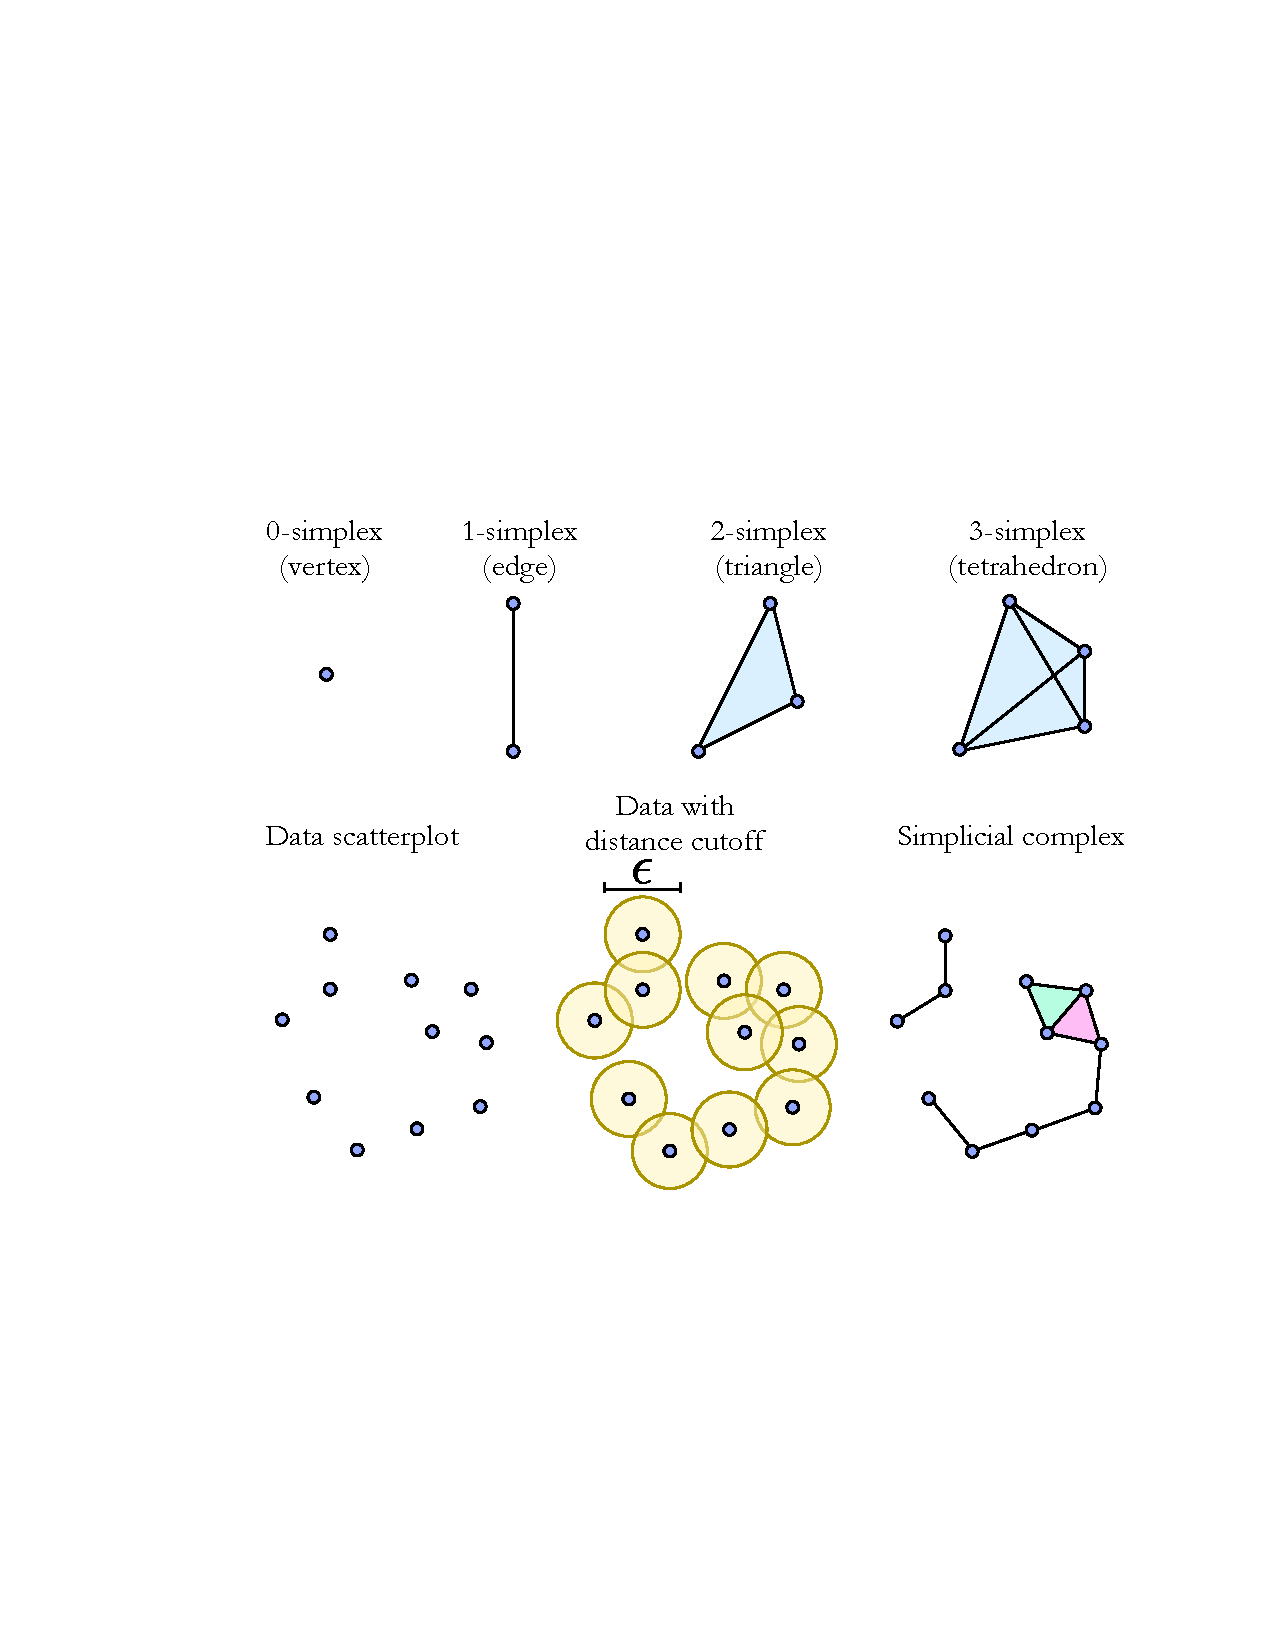
\includegraphics[clip=true, width=0.475\textwidth]{TDA_simplices_complex}
\captionspacefig \caption{(top) $k$-simplices\index{Simplex} are constructed as fully connected subsets of the data of different dimensions $k$. (bottom) A distance cutoff is applied to create edges within a scatterplot of raw data, from which the simplicial complex\index{Simplicial complex} is constructed. The shown example of a simplicial complex contains two 2-simplices (coloured triangles), and 6 1-simplices (edges). The final simplicial complex is highly dependent on the choice of cutoff $\epsilon$. In general, as $\epsilon$ is increased the complex will contain more simplices of higher dimension, since vertices will have more immediate neighbours.} \label{fig:TDA_simplex}	
\end{figure}

The first step in the algorithm is to construct the simplicial complex superposition state,
\begin{align}
\ket\psi_k^\epsilon = \frac{1}{\sqrt{|S_k^\epsilon|}} \sum_{s_k\in S_k^\epsilon} \ket{s_k},
\end{align}
where $s_k$ denotes a $k$-simplex from the simplicial complex $S_k^\epsilon$. This superposition can be constructed by employing a Grover search\index{Grover's algorithm} using a set-membership oracle function\index{Oracles},
\begin{align}
f_\epsilon(s_k) = \left\{ \begin{matrix}
 1, & \mathrm{if}\,\,s_k\in S_k^\epsilon \\
 0, & \mathrm{otherwise}
\end{matrix}\right.,
\end{align}
yielding quadratically enhanced efficiency in the simplicial complex state preparation.

From the superposition state, the uniform mixture of simplices state,
\begin{align}
\hat\rho_k^\epsilon = \frac{1}{|S_k^\epsilon|} \sum_{s_k\in S_k^\epsilon} \ket{s_k}\bra{s_k},
\end{align}
is easily prepared with the addition of CNOT gates and ancillary qubits\footnote{Using parallel CNOT gates one can transform an arbitrary superposition state into a redundantly encoded equivalent, \mbox{$\hat{U}_\mathrm{CNOTs}\sum_i \lambda_i \ket{\psi_i}\ket{0} \to \sum_i \lambda_i \ket{\psi_i}\ket{\psi_i}$}, following which tracing out the redundant copy takes us to its uniform mixture, \mbox{$\sum_i |\lambda_i|^2\ket{\psi_i}\bra{\psi_i}$}.}.

The quantum TDA algorithm then takes the simplicial complex mixed state and estimates the full set of Betti numbers by employing a phase-estimation algorithm\index{Phase estimation algorithm} (Sec.~\ref{sec:phase_est_alg}), which induces an exponential algorithmic runtime improvement. The full TDA algorithm is summarised in Alg.~\ref{alg:TDA}.

Performing the TDA across a range of $\epsilon$ yields a \textit{barcode}\index{Barcode} representation for the dataset's topology. Topological features which persist over large ranges of $\epsilon$ can then be regarded as robust features of the dataset, whereas ones which only persist over a small range of $\epsilon$ can be regarded as localised, non-persistent features, which might correspond to noise for example, and be filtered out prior to further analysis. The barcode representation thereby gives us an extremely robust characterisation of the topology of the data in a scale-dependent way.

As an example for how this type of technique might be applied, consider Facebook's\index{Facebook} user database. The distance metric might relate to how similar users' interests are, or how closely related they are via their friendship networks. Then examining the barcode representation of the data by scanning over $\epsilon$ would provide insight into the persistence and robustness of these relationships at different scales within the network. At different scales we could investigate topological relationships and features at the level of individuals, family or friendship networks, communities, common interest groups, between cities, across demographic characteristics, or between nations, for example.

\begin{table}[!htbp]
\begin{mdframed}[innertopmargin=3pt, innerbottommargin=3pt, nobreak]
\texttt{
function TDA(dataPoints):
\begin{enumerate}
	\item Implement a Grover search on the set of data-points with set-membership oracle function,
	\begin{align}
f_\epsilon(s_k) = \left\{ \begin{matrix}
 1, & \mathrm{if}\,\,s_k\in S_k^\epsilon \\
 0, & \mathrm{otherwise}
\end{matrix}\right.,
\end{align}
which prepares the simplicial complex superposition state,
\begin{align}
\ket\psi_k^\epsilon = \frac{1}{\sqrt{|S_k^\epsilon|}} \sum_{s_k\in S_k^\epsilon} \ket{s_k},
\end{align}
	\item Using ancillary qubits, CNOT gates and a trace-out operation, prepare the simplicial complex uniform mixed state,
	\begin{align}
\hat\rho_k^\epsilon = \frac{1}{|S_k^\epsilon|} \sum_{s_k\in S_k^\epsilon} \ket{s_k}\bra{s_k},
\end{align}
	\item Perform quantum phase-estimation on the simplicial complex mixed state.
	\item \comment{To do - show how Betti numbers are calculated. Formulas.}
	\item Algorithm has runtime,
\begin{align}
O(n^5/\delta),
\end{align}
for accuracy $\delta$.
\item $\Box$
\end{enumerate}
\begin{center}
\if 2\pubmode
	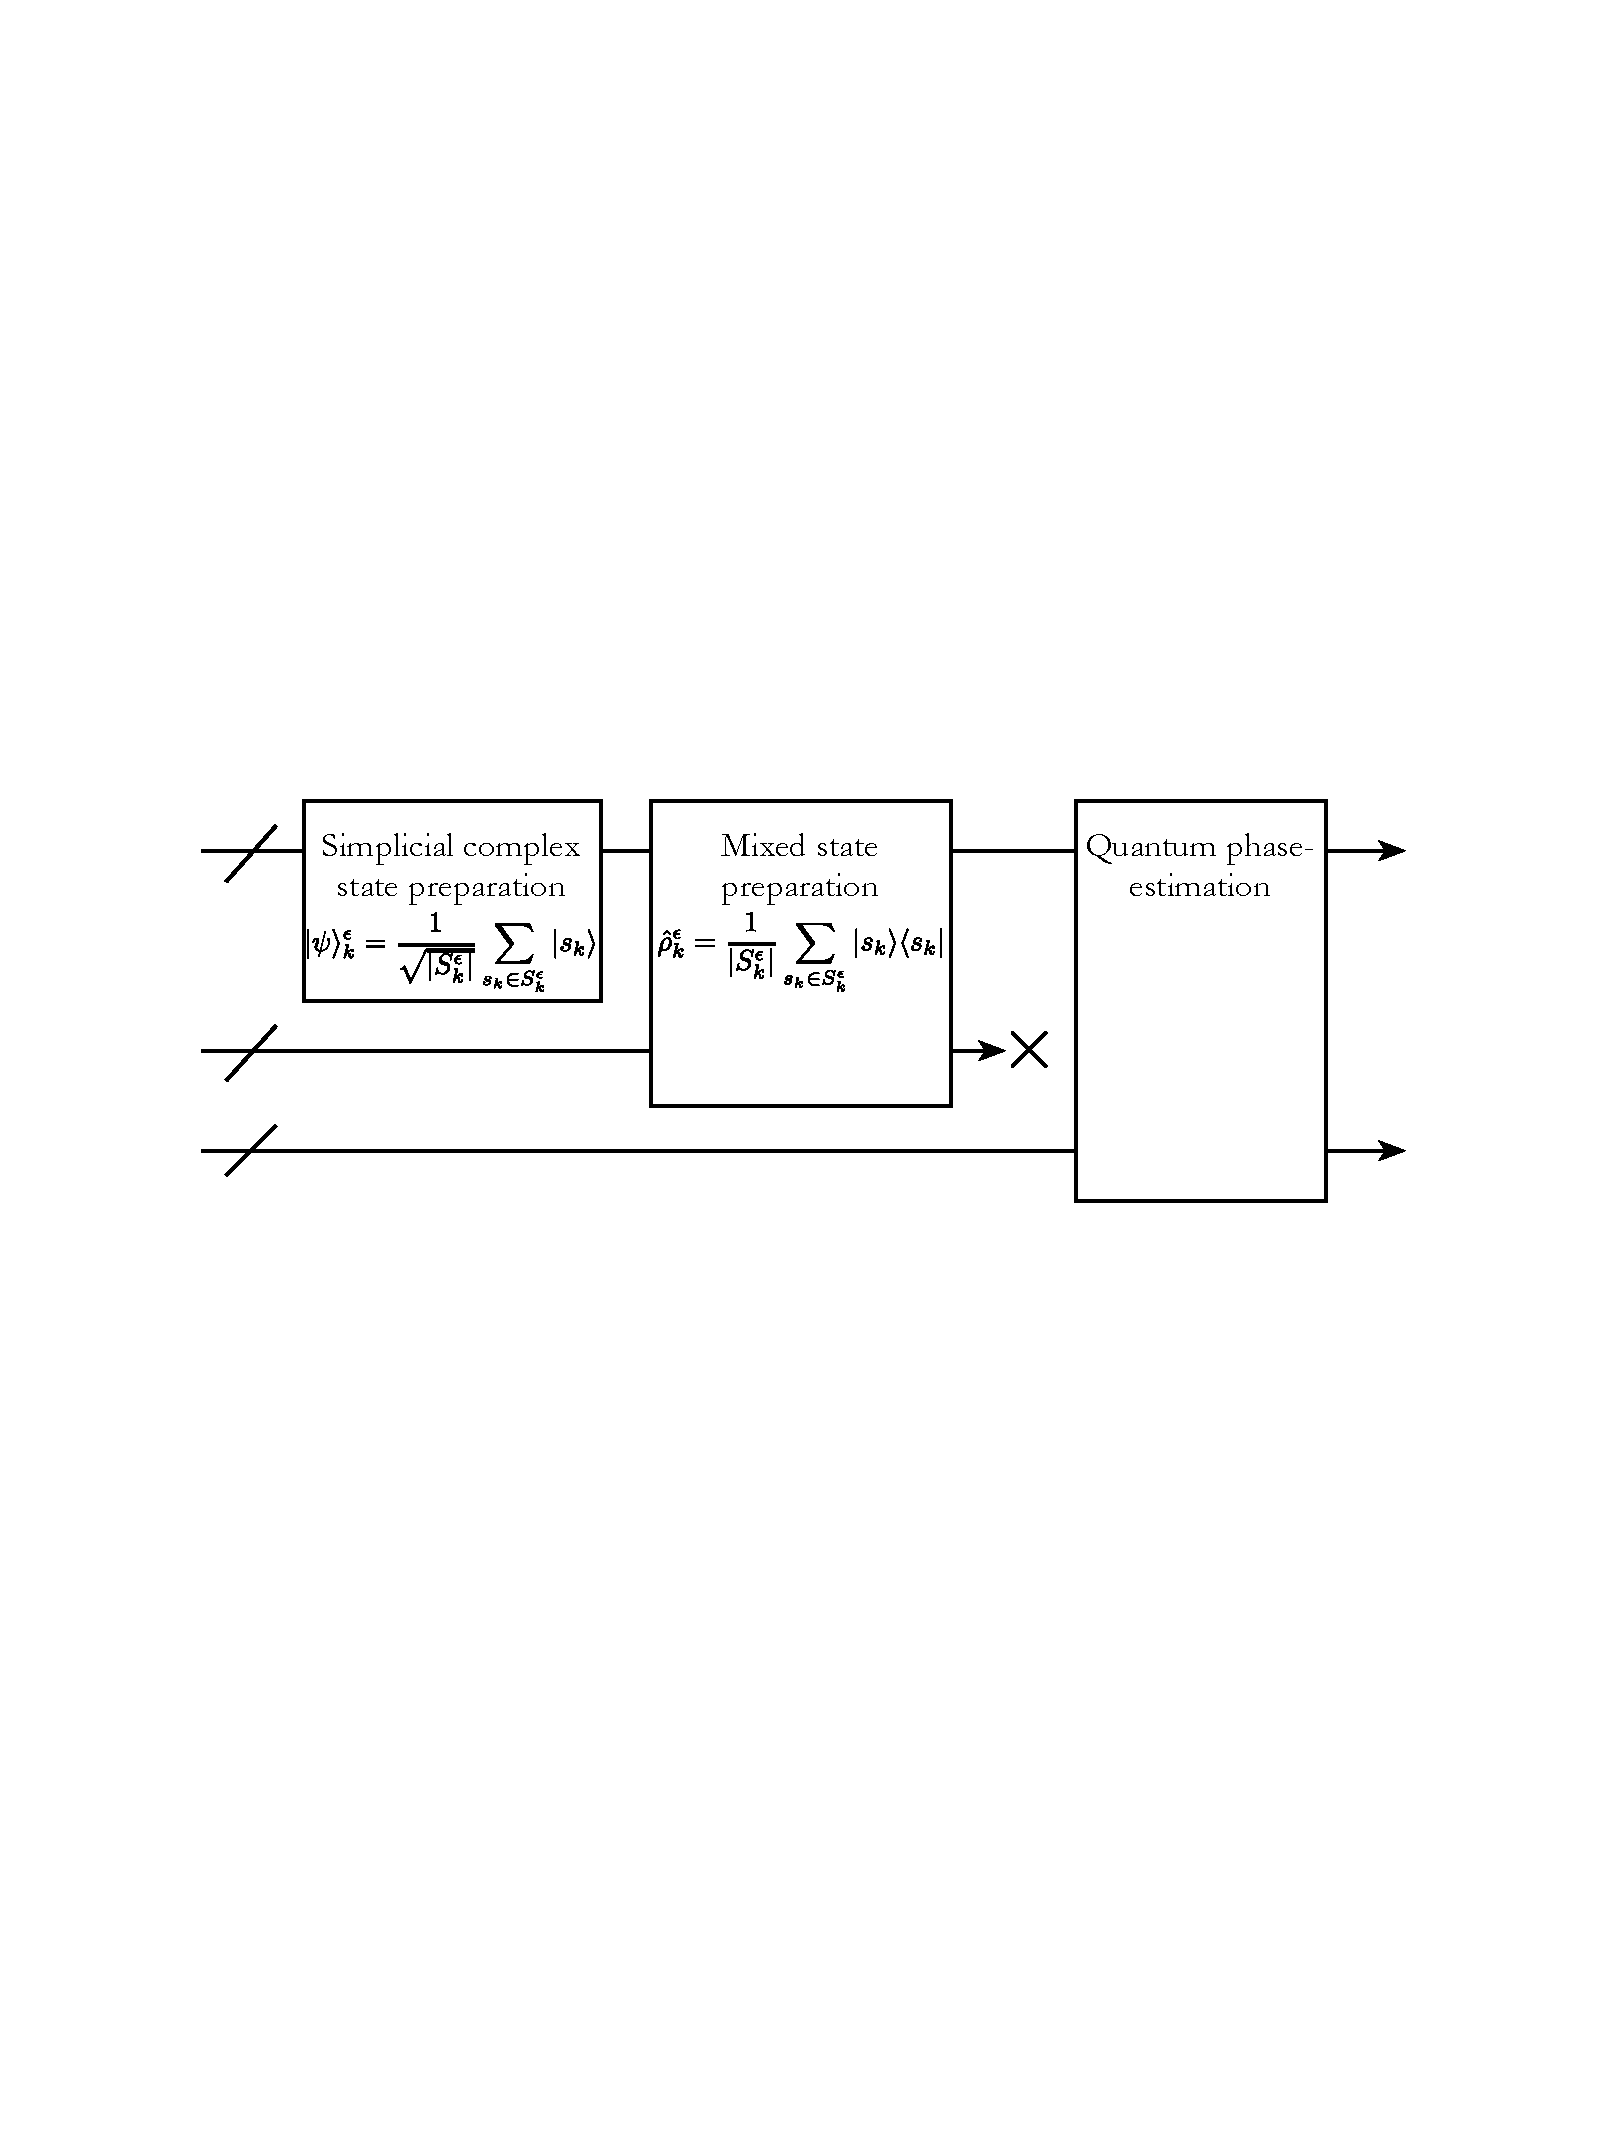
\includegraphics[clip=true, width=\textwidth]{TDA_circuit}
\else
	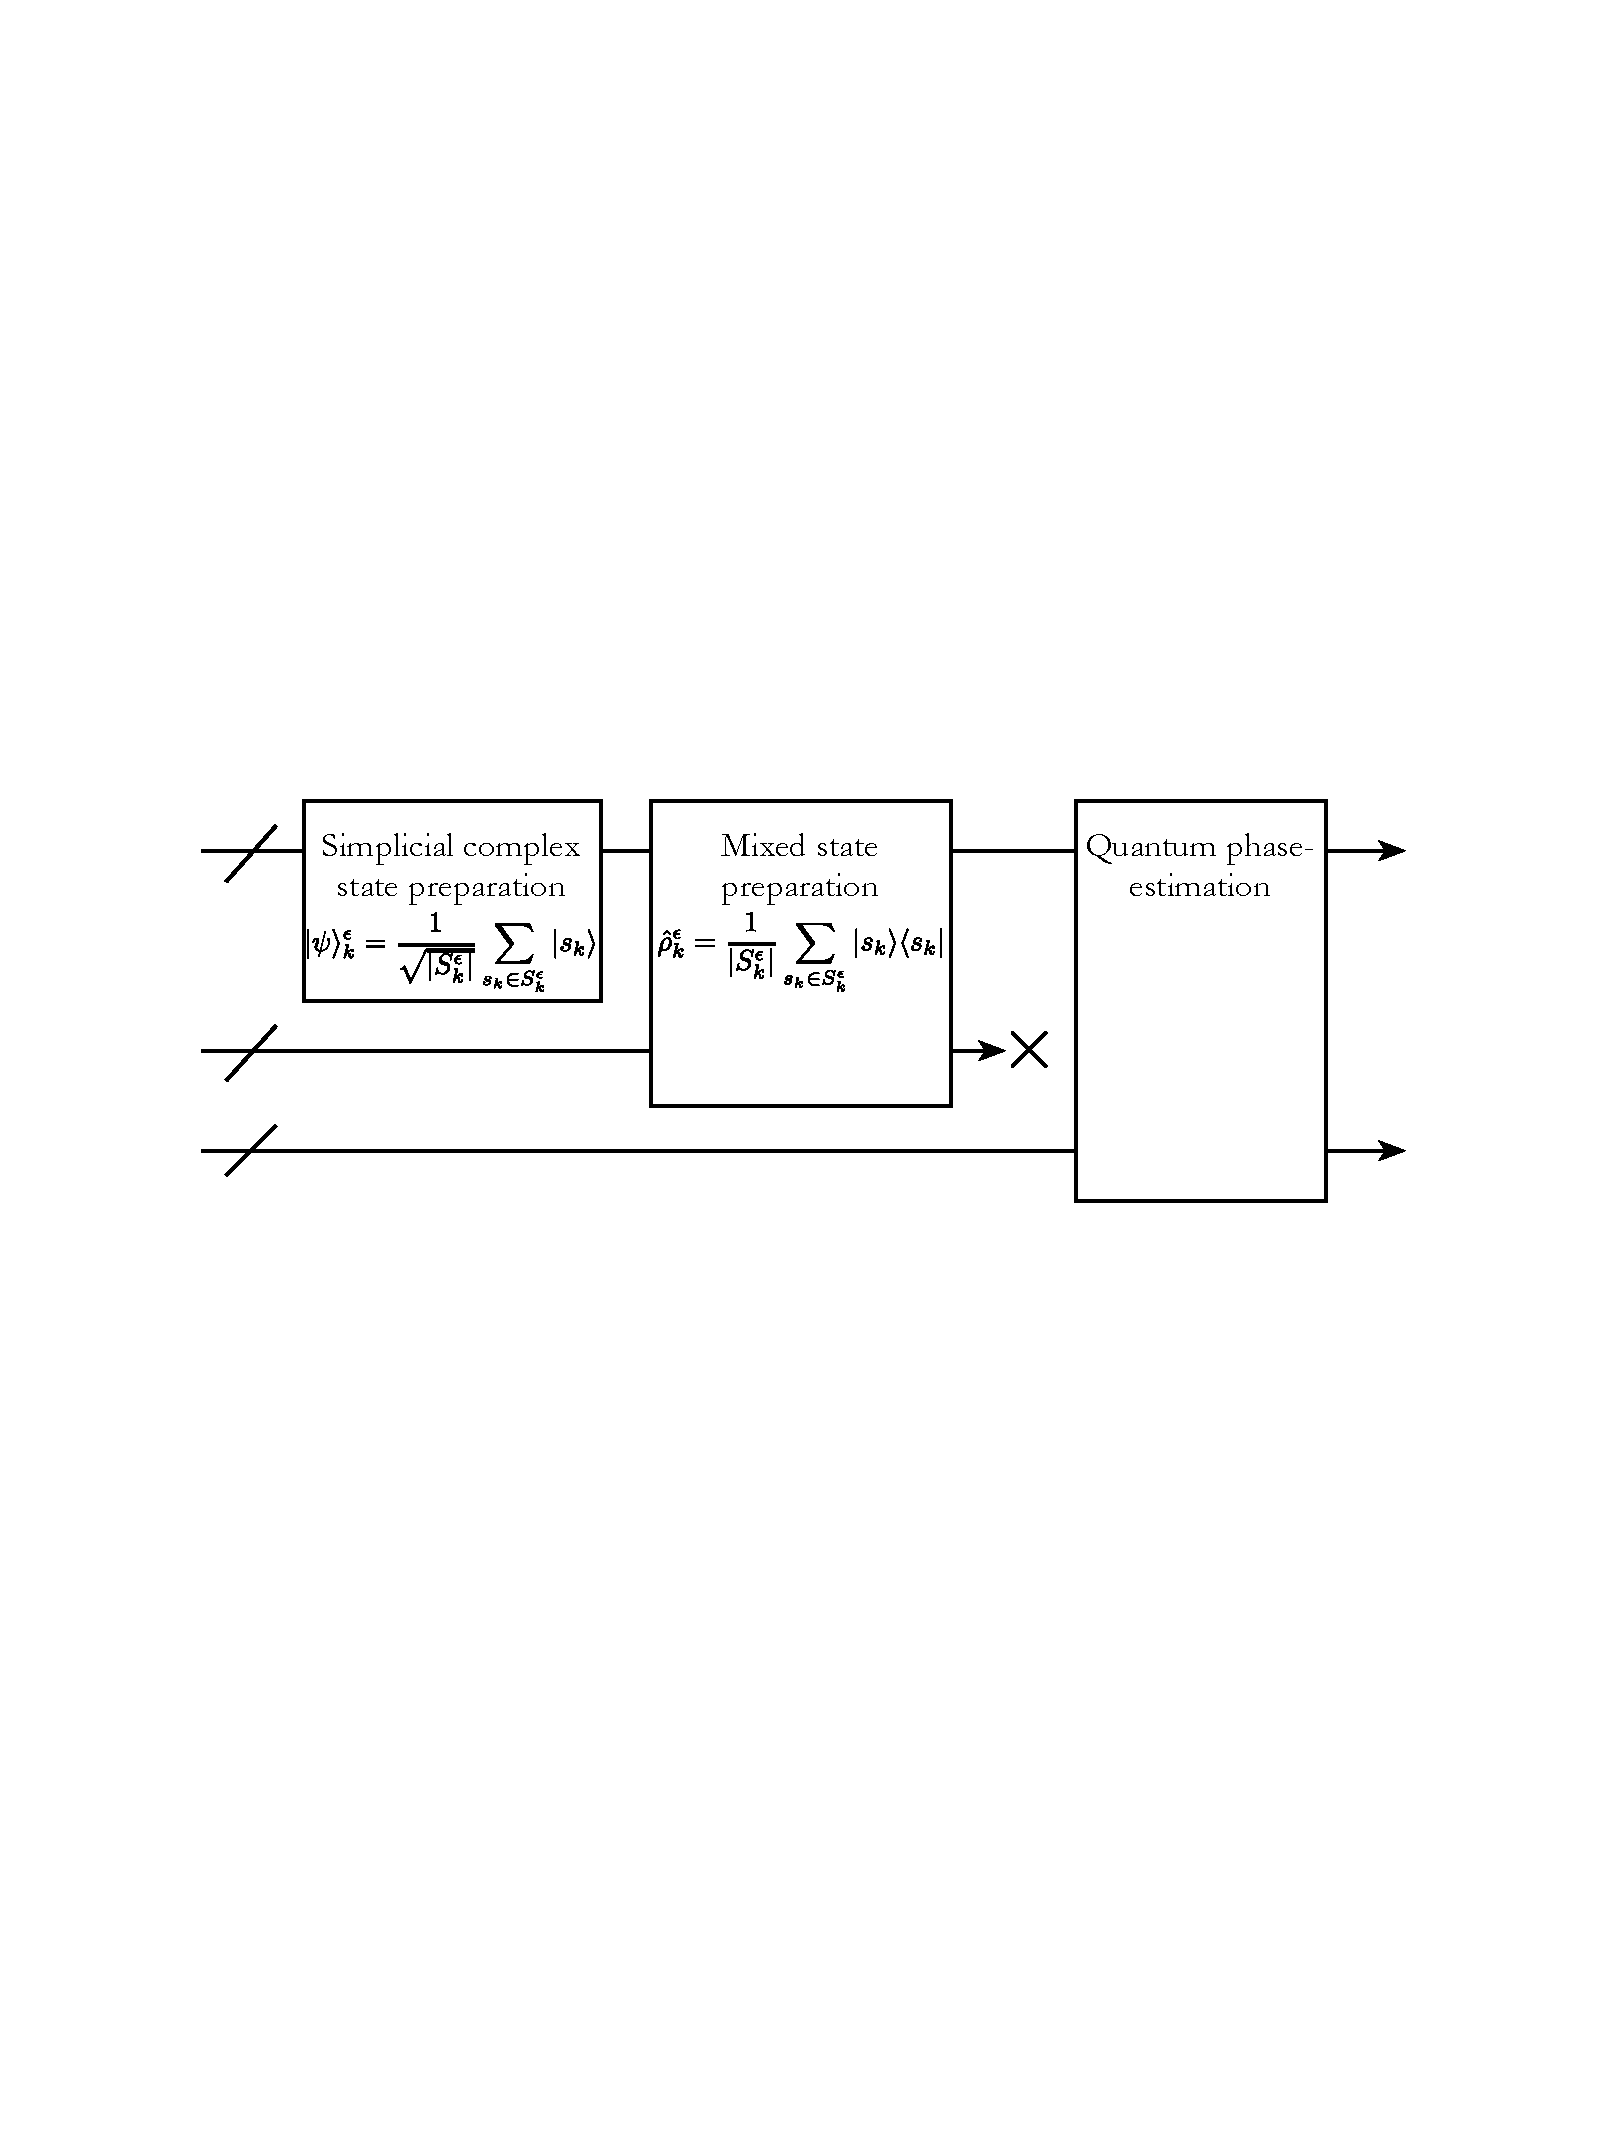
\includegraphics[clip=true, width=0.6\textwidth]{TDA_circuit}
\fi
\end{center}
}
\end{mdframed}
\captionspacealg \caption{Quantum topological data analysis algorithm for calculating Betti numbers.} \label{alg:TDA}
\end{table}

\comment{Finish mathematical details}

%
% Linear Systems
%

\subsection{Linear systems}\label{sec:linear_systems} \index{Linear systems}

\cite{bib:harrow2009quantum}

\comment{To do}

\comment{Example: recommendation algorithm where sampling the vector yields, with high probability, a recommendation that is a good one, without having to explicitly know the entire solution vector.}

%
% Sampling Problems
%

\subsection{Sampling problems}\index{Sampling problems}

The algorithms described previously are examples of \textit{decision problems}\index{Decision problems}, whereby the computation answers a question, providing a well-defined output for a well-defined input. Another entirely different class of problems are the so-called \textit{sampling problems}, whereby the goal is to accurately reproduce samples taken from some probability distribution. By their nature, these algorithms are statistical and generally their output cannot be associated with the answer to a decision problem. Nonetheless, despite being an entirely different category of problems, such problems reside in distinct sampling complexity classes, some of which are classically efficient to simulate, others not.

The simplest example of a classical sampling problem is the propagation of balls through a Galton board\index{Galton board}, as shown in Fig.~\ref{fig:galton_board}. This is a computationally easy problem, whose simulation requires only calculating a binomial distribution, which is classically straightforward.

\begin{figure}[!htbp]
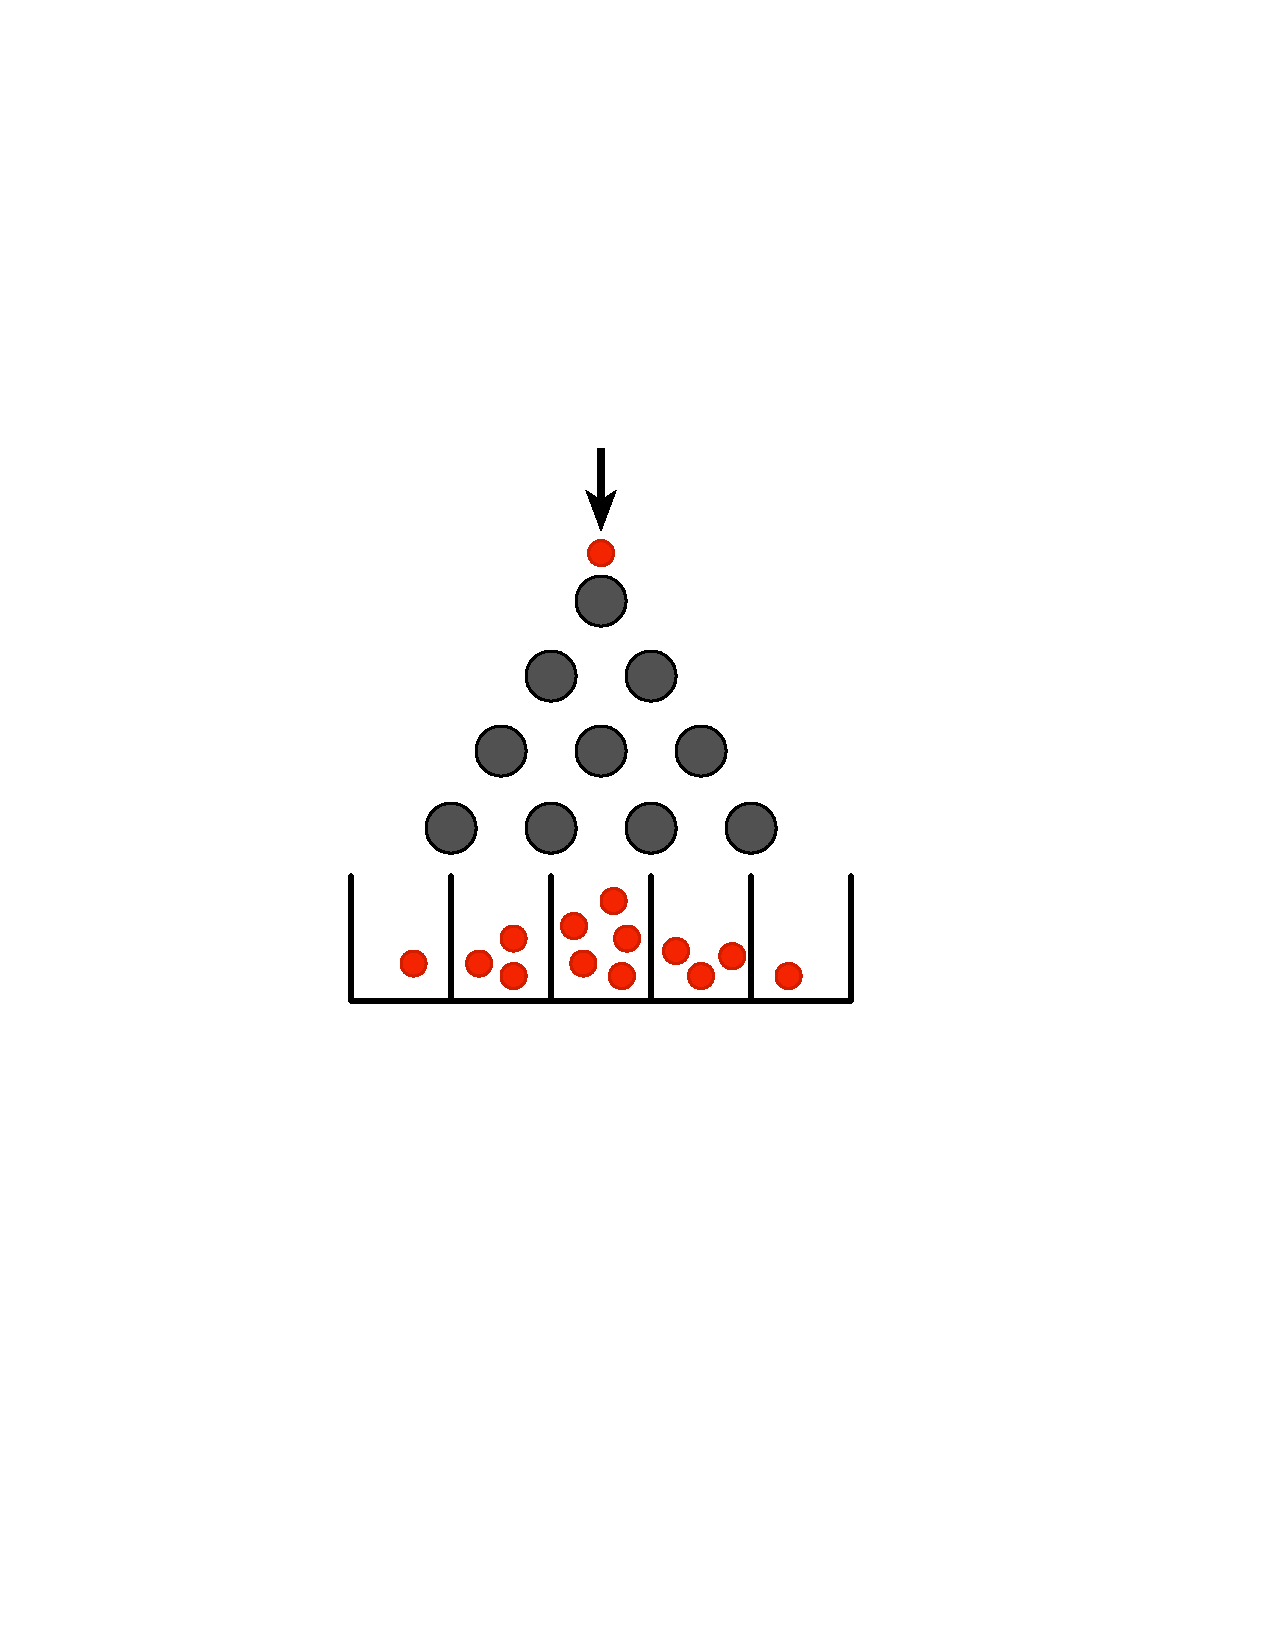
\includegraphics[clip=true, width=0.3\textwidth]{galton_board}
\captionspacefig \caption{The Galton board yields a very simple classical sampling problem. Balls (red) are input at the top and allowed to fall freely through the pyramid network of pegs (grey), at which balls bounce to the left or right with 50\% probability. At the output the balls are collected into buckets, which populate according to a binomial distribution\index{Binomial distribution}. The computational problem is to produce statistically accurate samples from such a device, which classically is efficiently implemented by sampling the binomial distribution.}	\label{fig:galton_board}\index{Galton board}
\end{figure}

An equivalent quantum sampling problem would be to replace the pegs in the Galton board with beamsplitters, and the balls with photons. Now we have an analogous problem, but defined in terms of photonic wave-function amplitudes rather than classical transition probabilities. When generalised to the multi-photon context, this problem turns into the so-called \textsc{BosonSampling}\index{Boson-sampling} problem, which is discussed in detail in Sec.~\ref{sec:BS}, a problem believed to not have an efficient classical simulation algorithm \cite{bib:AaronsonArkhipovBS}.

Countless other quantum sampling problems have been described. Most notably, the IQP (instantaneous quantum protocol)\index{Instantaneous quantum protocol (IQP)} sampling problem is a very simple prescription for a quantum algorithm that has been shown to likely be classically hard \cite{bib:BremnerIQP}.

Although not as obviously algorithmically useful as decision problems, sampling problems have received much interest owing to their generally very simple construction. For example, \textsc{BosonSampling} requires only single-photon inputs, evolved via a passive linear optics\index{Linear optics} beamsplitter network, and measured using photo-detection\index{Photo-detection}. IQP sampling requires only single-qubit Hadamard gates\index{Hadamard gate} and generalised multi-qubit controlled-phase gates\index{Generalised controlled-phase gates}\footnote{Generalised CZ gates are simply gates diagonal in the logical basis, where the diagonal elements are arbitrary phases, \mbox{$\hat{U}_\mathrm{CZ} = \mathrm{diag}(e^{i\theta_1},\dots,e^{i\theta_n})$}.}, thereby sampling from the logical state,
\begin{align}
\ket{\psi_\mathrm{out}} = \hat{H}^{\otimes n} \cdot \hat{U}_\mathrm{CZs} \cdot \hat{H}^{\otimes n} \ket{0}^{\otimes n}.	
\end{align}
Because CZ gates commute, they can be performed in parallel, giving the IQP circuit construction very low circuit depth\index{Circuit depth}. The IQP protocol is shown in Alg.~\ref{alg:IQP_samp}.

\begin{table}[!htbp]
\begin{mdframed}[innertopmargin=3pt, innerbottommargin=3pt, nobreak]
\texttt{
function IQPsampling():
\begin{enumerate}
    \item Prepare the $n$-qubit state,
    \begin{align}
    \ket{\psi_\mathrm{in}} = \ket{0}^{\otimes n}.
    \end{align} 
    \item Apply the $n$-qubit Hadamard transform,
    \begin{align}
	\hat{H}^{\otimes n}.
	\end{align}
    \item Apply some choice of generalised CZ gates,
	\begin{align}
	\hat{U}_\mathrm{CZs} = \mathrm{diag}(e^{i\theta_1},\dots,e^{i\theta_n}).
	\end{align}
	\item Apply another $n$-qubit Hadamard transform,
    \begin{align}
	\hat{H}^{\otimes n}.
	\end{align}
	\item The output state is,
	\begin{align}
		\ket{\psi_\mathrm{out}} = \hat{H}^{\otimes n} \cdot \hat{U}_\mathrm{CZs} \cdot \hat{H}^{\otimes n} \ket{0}^{\otimes n}.	
	\end{align}
	\item Measure all qubits in the computational basis, yielding bit-string $\vec{x}$, which occurs with probability,
	\begin{align}
		P_{\vec{x}} = |\langle \vec{x} | \hat{H}^{\otimes n} \cdot \mathrm{diag}(e^{i\theta_1},\dots,e^{i\theta_n}) \cdot \hat{H}^{\otimes n} \ket{0}^{\otimes n}|^2.
	\end{align}
	\item Repeat protocol $O(\mathrm{poly}(n))$ times.
	\item $\Box$
\end{enumerate}
\begin{align}
\Qcircuit @C=1em @R=1.6em {
    \lstick{\ket{0}} & \gate{\hat{H}} & \multigate{2}{\hat{U}_\mathrm{CZs}} & \gate{\hat{H}} & \meter \\
    \lstick{\vdots} & \gate{\hat{H}} & \ghost{\hat{U}_\mathrm{CZs}} & \gate{\hat{H}} & \meter \\
    \lstick{\ket{0}} & \gate{\hat{H}} & \ghost{\hat{U}_\mathrm{CZs}} & \gate{\hat{H}} & \meter \\
} \nonumber
\end{align}
}
\end{mdframed}
\captionspacealg \caption{The IQP sampling problem, which is believed to be a classically hard problem.} \label{alg:IQP_samp}
\end{table}

These reduced resource requirements makes both analysis and physical construction of some sampling problems far simpler than a universal quantum computer, yet nonetheless they implement computationally hard problems. For these reasons, many researchers regard non-universal sampling problems as being likely candidates for the first demonstration of quantum supremacy\index{Quantum supremacy}.